\section{Simulation results}

We compare performance of PSRL to UCRL2 \cite{jaksch2010near}, an optimistic algorithm with similar regret bounds. We use the benchmark example of \emph{RiverSwim} \cite{strehl2008analysis}, as well as several randomly generated MDPs. We provide results in both the episodic case, where the state is reset every $\tau=20$ steps, as well as the setting without episodic reset.

\begin{figure}[h!]
  \centering
    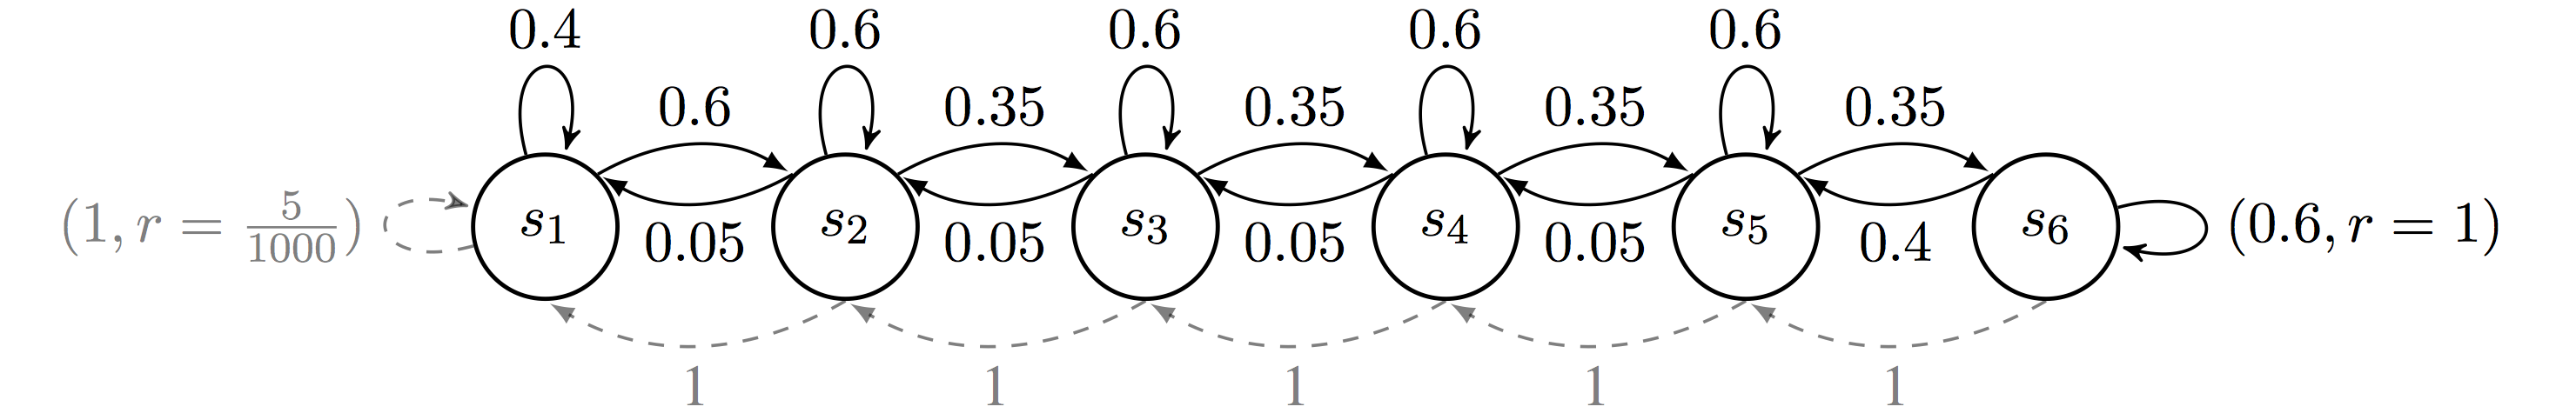
\includegraphics[width=0.9\textwidth]{Diagrams/RiverSwim}      
      \caption{\emph{RiverSwim} - continuous and dotted arrows represent the MDP under the actions ``right" and ``left".}
      \label{figure: RiverSwim}
\end{figure}

\emph{RiverSwim} consists of six states arranged in a chain as shown in Figure \ref{figure: RiverSwim}. The agent begins at the far left state and at every time step has the choice to swim left or right. Swimming left (with the current) is always successful, but swimming right (against the current) often fails. The agent receives a small reward for reaching the leftmost state, but the optimal policy is to attempt to swim right and receive a much larger reward. This MDP is constructed to require efficient exploration to obtain the optimal policy. For the random MDPs we sampled 10-state, 5-action environments according to the prior.

We express our prior in terms of Dirichlet and normal-gamma distributions over the transitions and rewards respectively.\footnote{These priors are conjugate to the multinomial and normal distribution, facilitating efficient posterior updating and sampling. We used the values $ \alpha=1/S , \mu=\sigma^2=1$ and pseudocount $n=1$ for a diffuse uniform prior.}
In both environments we perform 20 Monte Carlo simulations and compute the total regret over 10,000 time steps. We implement UCRL2 with $\delta =0.05$ and optimize the algorithm to take account of finite episodes where appropriate. PSRL outperformed UCRL2 across every environment, as shown in Table 1. In figure \ref{fig:RiverSwim}, we show regret through time across 50 Monte Carlo simulations to 100,000 timesteps in the \emph{RiverSwim} environment, PSRL's outperformance is quite extreme.

%\begin{table}[h!]
%\begin{center}
%\begin{tabular}{| c | c c | c c | }
%\hline
%				& Random MDP	& Random MDP	& \emph{RiverSwim} 	& \emph{RiverSwim} \\
%	Algorithm		& $\tau$ episodes	& $\infty$-horizon 	& $\tau$ episodes	& $\infty$-horizon 	\\
%\hline
%	PSRL		& $1.95 \times 10^5$& $2.25 \times 10^6$&$1.20 \times 10^2$	& $3.30 \times 10^2$ \\
%	UCRL2		&$8.07 \times 10^4$	& $1.26 \times 10^6$&$1.05 \times 10^0$	& $1.49 \times 10^0$ \\
%\hline
%\end{tabular}
%\end{center}
%\caption{Average rewards in simulation. PSRL outperforms UCRL2 across different environments.}
%\label{table:AveRewards}
%\end{table}

\begin{table}[h!]
\begin{center}
\caption{Total regret in simulation. PSRL outperforms UCRL2 across different environments.}
\begin{tabular}{| c | c c | c c | }
\hline
				& \emph{Random MDP}	& \emph{Random MDP}	& \emph{RiverSwim} & \emph{RiverSwim} \\
\emph{Algorithm}		& $\tau$\emph{-episodes}	& $\infty$\emph{-horizo}n 	& $\tau$\emph{-episodes}	& $\infty$\emph{-horizon} 	\\
\hline
	PSRL		& $1.04 \times 10^4$& $7.30 \times 10^3$&$6.88 \times 10^1$	& $1.06 \times 10^2$ \\
	UCRL2		&$5.92 \times 10^4$	& $1.13 \times 10^5$&$1.26 \times 10^3$	& $3.64 \times 10^3$ \\
\hline
\end{tabular}
\end{center}
\label{table: AveRewards}
\end{table}

\subsection{Learning in MDPs without episodic resets}
The majority of practical problems in reinforcement learning can be mapped to repeated episodic interactions for some length $\tau$. Even in cases where there is no actual reset of episodes, one can show that PSRL's regret is bounded against all policies which work over horizon $\tau$ or less\cite{brafman2003r}. Choosing $\tau$ large enough from prior knowledge, we can compete with the optimal policy for any given problem. Alternatively, any setting with discount factor $\alpha$ can be learned to arbitrary accuracy for $\tau \propto (1-\alpha)^{-1}$.

\begin{figure}[h!]
\centering
\begin{subfigure}{.5\textwidth}
  \centering
  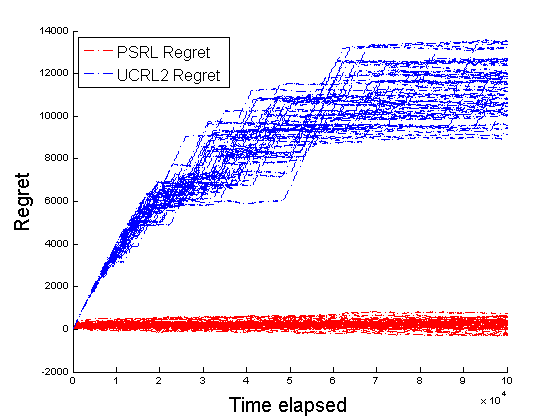
\includegraphics[width=1\linewidth]{Diagrams/combinedGraph.png}
  \caption{PSRL outperforms UCRL2 by large margins}
  \label{fig:sub1}
\end{subfigure}%
\begin{subfigure}{.5\textwidth}
  \centering
  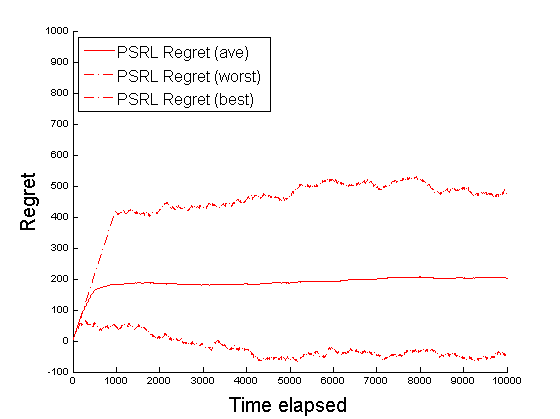
\includegraphics[width=1\linewidth]{Diagrams/psrlGraphShort.png}
  \caption{PSRL learns quickly even with a misspecified prior}
  \label{fig:sub2}
\end{subfigure}
\caption{Simulated regret on the $\infty$-horizon \emph{RiverSwim} environment.}
\label{fig:RiverSwim}
\end{figure}

Nevertheless, for infinite-horizon and undiscounted problems artificially imposing a $\tau$ too small risks overlooking an optimal policy operating over a larger timeframe, whereas a $\tau$ too large may learn slowly. One particularly appealing feature of UCRL2 \cite{jaksch2010near} and REGAL \cite{bartlett2009regal}  is that they learn an optimal timeframe from experience, and replace the factor $\tau$ in \eqref{eq: high probability regret bound} by the diameter and span of the underlying MDP respectively. They both accomplish this by allowing the length of their episodes of fixed policy to vary depending upon the states and actions visited. A new episode is begun, and a policy computed, only when the total visits to any state-action pair is doubled, as opposed to fixed $\tau$-length intervals.

We can apply this same rule for episodes to PSRL, allowing the algorithm to learn more quickly initially, while eventually exploring policies over arbitrarily large timeframes. As shown in figure \ref{fig:RiverSwim} this implementation performs far better than UCRL2, even with a grossly misspecified prior. We see that, while UCRL2's regret grows with the worst case $T$-dependence of $\sqrt{T}$, PSRL performs much better than these bounds and settles upon the optimal policy after only 500 time steps on average.

At present, our analysis for deterministic $\tau$ episodes does not follow through to this infinite horizon extension, since the length episodes of fixed policy is no longer independent observations $H_{t_k}$. For this reason, we are unable to state an equivalent result to (\ref{eq: from Delta to Delta tilde}) relating optimal rewards to those observed by the agent. However, where the optimal average reward of the sampled MDP $M_k$ is uncorrelated with episode length, we can derive results analogous to \cite{jaksch2010near,bartlett2009regal}: that expected regret is $\tilde{O}(S \sqrt{AT \Exp[\Psi^2]})$ where $\Psi$ is the span of bias vector of the optimal MDP $M^*$.


